% This file was created with tikzplotlib v0.10.1.post5.
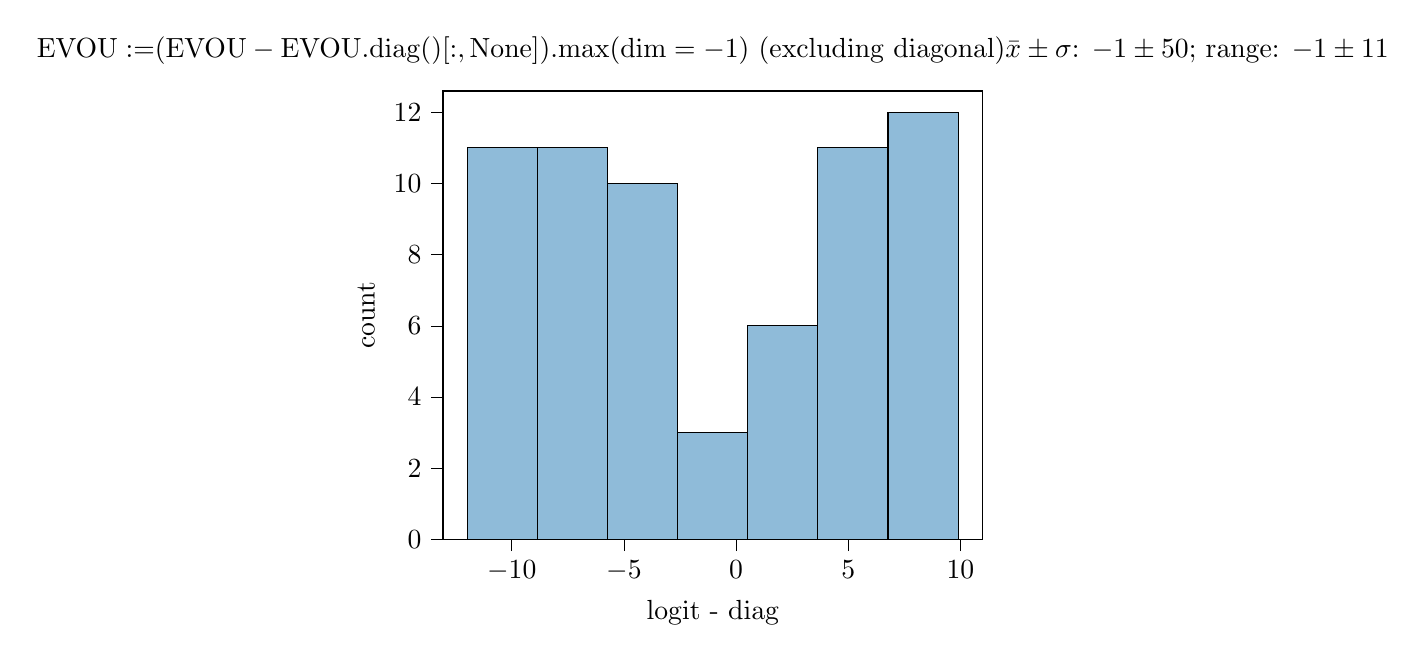
\begin{tikzpicture}

\definecolor{darkgray176}{RGB}{176,176,176}
\definecolor{steelblue31119180}{RGB}{31,119,180}

\begin{axis}[
tick align=outside,
tick pos=left,
title={\(\displaystyle \mathrm{EVOU} := \WE \WV \WO\WU \)\\
\(\displaystyle (\mathrm{EVOU} - \mathrm{EVOU}\mathrm{.diag}()[:,\mathrm{None}])\mathrm{.max}(\mathrm{dim}=-1)\) (excluding diagonal)\\
\(\displaystyle \bar{x}\pm\sigma\): \(\displaystyle -1 \pm 50\); range: \(\displaystyle -1 \pm 11\)},
x grid style={darkgray176},
xlabel={logit - diag},
xmin=-13.0643480300903, xmax=10.9897974014282,
xtick style={color=black},
xtick={-15,-10,-5,0,5,10,15},
xticklabels={
  \(\displaystyle {\ensuremath{-}15}\),
  \(\displaystyle {\ensuremath{-}10}\),
  \(\displaystyle {\ensuremath{-}5}\),
  \(\displaystyle {0}\),
  \(\displaystyle {5}\),
  \(\displaystyle {10}\),
  \(\displaystyle {15}\)
},
y grid style={darkgray176},
ylabel={count},
ymin=0, ymax=12.6,
ytick style={color=black},
ytick={0,2,4,6,8,10,12,14},
yticklabels={
  \(\displaystyle {0}\),
  \(\displaystyle {2}\),
  \(\displaystyle {4}\),
  \(\displaystyle {6}\),
  \(\displaystyle {8}\),
  \(\displaystyle {10}\),
  \(\displaystyle {12}\),
  \(\displaystyle {14}\)
}
]
\draw[draw=black,fill=steelblue31119180,fill opacity=0.5] (axis cs:-11.9709777832031,0) rectangle (axis cs:-8.84706279209682,11);
\draw[draw=black,fill=steelblue31119180,fill opacity=0.5] (axis cs:-8.84706279209682,0) rectangle (axis cs:-5.72314780099051,11);
\draw[draw=black,fill=steelblue31119180,fill opacity=0.5] (axis cs:-5.72314780099051,0) rectangle (axis cs:-2.59923280988421,10);
\draw[draw=black,fill=steelblue31119180,fill opacity=0.5] (axis cs:-2.59923280988421,0) rectangle (axis cs:0.524682181222099,3);
\draw[draw=black,fill=steelblue31119180,fill opacity=0.5] (axis cs:0.524682181222099,0) rectangle (axis cs:3.6485971723284,6);
\draw[draw=black,fill=steelblue31119180,fill opacity=0.5] (axis cs:3.6485971723284,0) rectangle (axis cs:6.77251216343471,11);
\draw[draw=black,fill=steelblue31119180,fill opacity=0.5] (axis cs:6.77251216343471,0) rectangle (axis cs:9.89642715454102,12);
\end{axis}

\end{tikzpicture}
